\chapter{Enforcing Constraints}
\label{ch:enforcing_constraints}

This chapter explains how the constraints are expressed and validated in the tool using the definitions of the rules as well as by applying the rules to a modeled example system. The constraints are divided into three distinct categories. The first category contains the constraints that are possible to express in ArchUnit as-is. The second category describes constraints that are enforceable with the help of additional information in source code. The third and final category details constraints that require an extension of ArchUnit to be possible to enforce.

\section{Running example}
We modeled a toy system, BlogWeb, and use it as a running example for this chapter. By no means is this example meant to be a realistic application, but is instead used to showcase our constraints.
A UML class diagram of BlogWeb is illustrated in Figure~\ref{fig:toy_application}.

%However, a toy system called \textit{BlogWeb} has been modeled to allow us to showcase a specific example for each constraint. BlogWeb is by no means intended to be a complex or complete system, but rather big enough to provide the functionality to support the constraints.

\begin{figure}
    \centering
    \captionsetup{justification=centering}
    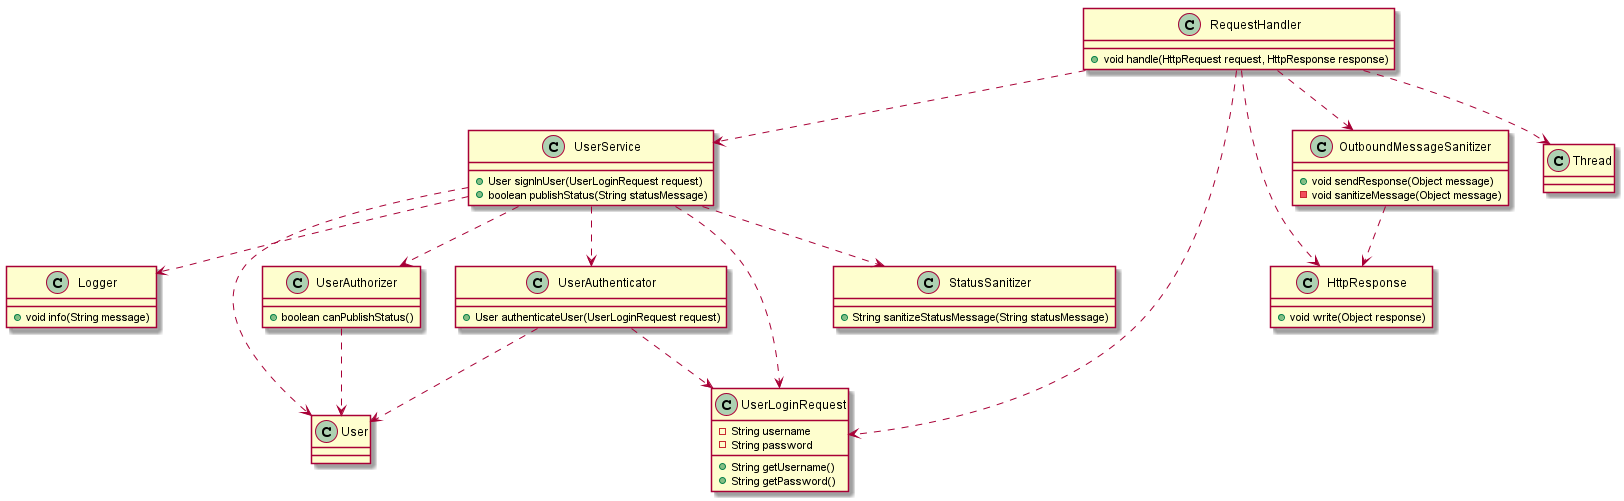
\includegraphics[width=\textwidth]{figure/ToyApp.png}
    \caption
        [UML class diagram of the toy system BlogWeb]
        {A UML class diagram of the toy system BlogWeb. Zoom in to read the labels, or see full-scale version in Appendix~\ref{apx:blogweb}.}
    \label{fig:toy_application}
\end{figure}

BlogWeb is, as the name suggests, a blog website providing users with the ability to publish statuses to their blogs. Being a website means that the system receives actions to execute via HTTP requests. These requests are received by the RequestHandler and are forwarded to the UserService, which provides public methods for sign in and publishing a status update. The UserService depends on UserAuthorizer and UserAuthenticator which implement the logic for authorization and authentication. The UserService also uses the Logger to perform the necessary logging of user requests. StatusSanitizer is used to sanitize the status updates received by users before they are stored while OutBoundMessageSanitizer is responsible for sanitizing responses. Finally, as the RequestHandler may serve several users at once, a thread is spawned for each request to make the execution concurrent. 


\section{Support in ArchUnit as-is}\label{sec:as-is}
ArchUnit contains an extensive vocabulary for expressing architectural constraints in a sentence-like manner, as exemplified in Section~\ref{archunit-back-section}. In situations where the standard vocabulary is insufficient for expressing a constraint, there is a possibility to define custom predicates and conditions over any given construct. These can be supplied as arguments to the \texttt{that()} and \texttt{should()} methods. Custom predicates and conditions are used extensively in our implementation, as will be made apparent in the following sections.

%\begin{center}
%\begin{minipage}{0.90\linewidth}
%\begin{lstlisting}[caption={Example of a rule that is expressed with the standard vocabulary.}, %captionpos=b, label=lst:standard_vocabulary, numbers=left]
%ArchRule rule = classes()
%    .that().resideInAPackage("..internal..")
%    .should().onlyBeAccessed().byAnyPackage("..mediator..");
%\end{lstlisting}
%\end{minipage}
%\end{center}

% in ArchUnit are composed of three parts. The first part (line 1 in Listing~\ref{lst:standard_vocabulary}) is the type of Java constructs that should be inspected; namely classes, fields or methods. The second part (line 2) is a predicate that is used to filter for constructs related to the constraint. The third part (line 3) describes the logical condition that must hold true for all of the selected constructs. In short, rules are generally expressed as sentences of the form \say{The \textbf{constructs} that match \textbf{predicate} should fulfill \textbf{condition}.}

%These constraints are generally composed of three parts: a construct, a predicate and a condition. The construct defines the type of Java construct that should be inspected, and includes classes, methods, fields and constructors. The predicate then selects a subset of these constructs, for which the condition must hold true.



\subsection{Constraint 1: Log all security events}
% Description
The definition of the architectural rule related to constraint 1 can be seen in Listing~\ref{lst:constraint_1_impl}. This constraint is expressed with the assumption that there are services, in the form of classes, which are responsible for performing security related events. Every publicly accessible method in such a service is assumed to perform a security event and must therefore contain a call to the logging facility for accountability purposes.

\begin{minipage}{\linewidth}
\begin{lstlisting}[caption={Rule definition for constraint 1.}, captionpos=b, label=lst:constraint_1_impl, numbers=left]
ArchRule logSecurityEvents(
        DescribedPredicate<? super JavaClass> securityServicesDescriptor,
        Class<?> logger) {
    return methods()
        .that().haveModifier(JavaModifier.PUBLIC)
        .and().areDeclaredInClassesThat(securityServicesDescriptor)
        .should(callMethod(declaredIn(logger)));
}
\end{lstlisting}
\end{minipage}

% Rule definition
The predicate that selects the security services, and the class that is responsible for logging, are passed as arguments to the architectural rule. Hence, there is no need for adding information to the source code of the target system. Furthermore, by using a predicate to select the security services, the developer is left with some flexibility in how they decide to apply the constraint to a system. As opposed to a plain list of classes, a predicate can match all classes belonging to a specific package or following a set naming scheme, minimizing the need for revisiting the constraint as the system evolves. The logger, on the other hand, is described as a single class, meaning that all events must be logged with the same global logger.

% Applied to toy app
In BlogWeb, illustrated in Figure~\ref{fig:toy_application}, the logging facility is the class named \texttt{Logger} while the only security service is the \texttt{UserService} class. An application of the constraint on this system can be as simple as the one shown in Listing~\ref{lst:constraint_1_toy}.

\begin{minipage}{\linewidth}
\begin{lstlisting}[caption={Application of constraint 1 to BlogWeb.}, captionpos=b, label=lst:constraint_1_toy, numbers=left]
@ArchTest
ArchRule logSecurityEvents = SecArchUnit
    .logSecurityEvents(type(UserService.class), Logger.class);
\end{lstlisting}
\end{minipage}

\subsection{Constraint 2: Enforce AuthN/AuthZ at single point}
% Description
The definition of the second constraint is detailed in Listing~\ref{lst:constraint_2_impl}.
This constraint is defined in terms of two concepts: an authentication point and an authentication enforcer. Authentication is performed through a method call to the authentication enforcer, which is a class whose sole responsibility is to authenticate an actor. This call should only occur at the authentication point for the sake of ensuring a uniform authentication mechanism throughout the system. Authorization is enforced in the same manner, with the concepts of an authorization point and an authorization enforcer.

\begin{minipage}{\linewidth}
\begin{lstlisting}[caption={Rule definitions for constraint 2.}, captionpos=b, label=lst:constraint_2_impl, numbers=left]
ArchRule enforceAuthenticationAtCentralPoint(
        Class<?> authenticationPoint,
        Class<?> authenticator) {
    return CompositeArchRule.of(
        theClass(authenticationPoint)
            .should(callMethod(declaredIn(authenticator)))
    ).and(
        methods()
            .that().areDeclaredIn(authenticator)
            .should(onlyBeAccessedBy(authenticationPoint))
    );
}

ArchRule enforceAuthorizationAtCentralPoint(
        Class<?> authorizationPoint,
        Class<?> authorizer) {
    return enforceAuthenticationAtCentralPoint(
        authorizationPoint,
        authorizer
    );
}
\end{lstlisting}
\end{minipage}

% Rule definition
The constraint is defined as two separate rules, one for authentication and one for authorization. This is purely for the sake of clarity, as their implementations are identical.

% Applied to toy app
In BlogWeb, the authentication and authorization points are both situated in the \texttt{UserService} class while authentication and authorization are enforced by the classes \texttt{UserAuthenticator} and \texttt{UserAuthorizer} respectively. The application of the rule can be seen in Listing~\ref{lst:constraint_2_toy}.

\begin{minipage}{\linewidth}
\begin{lstlisting}[caption={Application of constraint 2 to BlogWeb.}, captionpos=b, label=lst:constraint_2_toy, numbers=left]
@ArchTest
ArchRule enforceAuthentication = SecArchUnit
    .enforceAuthenticationAtCentralPoint(UserService.class, UserAuthenticator.class);

@ArchTest
ArchRule enforceAuthorization = SecArchUnit
    .enforceAuthorizationAtCentralPoint(UserService.class, UserAuthorizer.class);
\end{lstlisting}
\end{minipage}

\subsection{Constraint 3: Messages are sent from a central point}
% Description
The rule definition of the third constraint can be seen in Listing~\ref{lst:constraint_3_impl}.
This constraint dictates that all outbound messages are sent from a central sending point. The intent is to have a single point that handles output sanitization or performs other safety checks on messages before they are sent. 

\begin{minipage}{\linewidth}
\begin{lstlisting}[caption={Rule definition for constraint 3.}, captionpos=b, label=lst:constraint_3_impl, numbers=left]
ArchRule sendOutboundMessagesFromCentralPoint(
        Class<?> sendingPoint,
        DescribedPredicate<? super JavaClass> senderDescriptor) {
    return methods()
        .that().areDeclaredInClassesThat(senderDescriptor)
        .and(haveAtLeastOneParameter)
        .should(onlyBeAccessedBy(sendingPoint));
}
\end{lstlisting}
\end{minipage}

% Rule definition
The act of sending a message is defined as a method call to a sender with at least one argument, which is assumed to contain the message contents. The reasoning behind this distinction, and why not all accesses are constrained, is that any class should be allowed to create and pass around a sender instance without violating the constraint.
Since there can be multiple sender classes in a system, e.g. one for HTTP requests and one for SMTP messages, the rule accepts a predicate that can select all these sender classes.

% Applied to toy app
Listing~\ref{lst:constraint_3_toy} showcases how the constraint can be applied to BlogWeb. In this system, there is a single sender class \texttt{HttpResponse}, responsible for returning a response to a client. The central sending point is the \texttt{OutboundMessageSanitizer} class. 

\begin{minipage}{\linewidth}
\begin{lstlisting}[caption={Application of constraint 3 to BlogWeb.}, captionpos=b, label=lst:constraint_3_toy, numbers=left]
@ArchTest
ArchRule centralSendingPoint = SecArchUnit
    .sendOutboundMessagesFromCentralPoint(
        OutboundMessageSanitizer.class,
        type(HttpResponse.class)
    );
\end{lstlisting}
\end{minipage}




\section{Adding information to source code}

Some of our constraints require that the developer adds additional information to the source code. In some cases, this information is simply an indicator that says something about an entire class. Naming the class with a specific prefix or suffix is one approach to accomplish this. Another approach is to implement an empty interface, which is the technique used with Java's \texttt{Serializable}\footnote{\url{https://docs.oracle.com/javase/7/docs/api/java/io/Serializable.html}} interface. 

In other cases, however, the information may be related to specific fields or methods of arbitrary signatures. For the purposes of flexibility and minimizing the obtrusiveness of our approach, any extra information is expressed in the form of annotations. These can be applied to classes, fields, methods and parameters without changing the underlying architecture of the system.

The need for additional information within the source code becomes apparent in the case where a class contains public methods with varying degrees of security requirements. A typical example is found in constraint 4, where a class is responsible for handling user input. Using the broader predicate of entire classes (described in Section~\ref{sec:as-is}) would not allow the constraint to be limited to the specific constructors or methods within the class that receive user input, and ensure that each of these perform proper sanitation. Thus, annotations provide the granularity needed to limit the scope of a constraint to the applicable code units only.

\subsection{Constraint 4: Validate user input}
The rule definition of constraint 4 can be seen in Listing~\ref{lst:constraint_4_impl}.
User input comes in many forms, and therefore, it is impossible to define a single algorithm to properly validate every single type. The problem grows further as queries (such as SQL) or other types of processed data (such as XML), each with its own set of grammar, are often formed using strings. As a consequence, the implemented constraint is more abstract as it checks whether a class that receives user input is said to either perform validation on its own or delegate the task another method. In total, three distinct cases conforming to the constraint were considered: 

\begin{enumerate}
    \item \textit{Method A} is annotated with both \textbf{UserInput} and \textbf{InputValidator}.
    
    \item \textit{Method A} is annotated with \textbf{UserInput} and calls a \textit{method B} that is annotated with \textbf{InputValidator}.
    
    \item \textit{Method A} is annotated with \textbf{UserInput} and is only called by methods that are annotated with \textbf{InputValidator}.
\end{enumerate}

\begin{minipage}{\linewidth}
\begin{lstlisting}[caption={Rule definition for constraint 4.}, captionpos=b, label=lst:constraint_4_impl, numbers=left]
ArchRule validateUserInput() {
    return codeUnits()
        .that().areAnnotatedWith(UserInput.class)
        .should(performDirectOrIndirectValidation);
}
\end{lstlisting}
\end{minipage}

As shown in Listing~\ref{lst:constraint_4_impl}, the \textbf{UserInput} annotation is used on line 3 to limit the set of applicable code units, whereas \texttt{performDirectOrIndirect\-Validation} is a custom condition that implements the logic to ensure that at least one of the three cases outlined above is satisfied. The full definition of this condition can be seen in Listing~\ref{lst:constraint_4_condition}.

In BlogWeb, a user publishes a status update in the form of a string that the UserService class receives. The status is then passed to the StatusSanitizer class, where it is validated. The affected methods of each class are marked with the appropriate annotation, as shown in Figure~\ref{fig:validate_input_toy_system}. If the two annotations were to be added, without a call from the relevant method in the \texttt{UserService} class to the \texttt{StatusSanitizer}, the rule would fail and mark it as a violation of the constraint.

\begin{figure}
    \centering
    \captionsetup{justification=centering}
    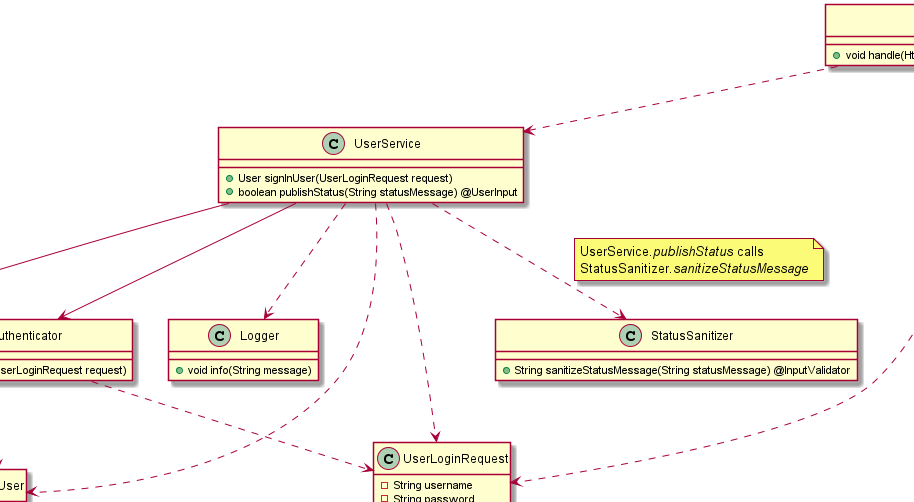
\includegraphics[width=\textwidth]{figure/toyexamples/validate_input_toy_system.png}
    \caption
        [Applying constraint 4 to BlogWeb]
        {Applying constraint 4 to the model of BlogWeb using added annotations on the UserService and StatusSanitizer class.}
    \label{fig:validate_input_toy_system}
\end{figure}

\subsection{Constraint 5: Restrict thread spawning}
The implementation of constraint 5 can be seen in Listing~\ref{lst:constraint_5_impl}.
While there are many ways computer resources can be exhausted, this constraint focuses on preventing the exhaustion of CPU time and memory specifically through the creation of new threads and processes. As such, every block of code that contains a call to the \texttt{start()} method of a \texttt{Thread}\footnote{\url{https://docs.oracle.com/javase/7/docs/api/java/lang/Thread.html}} or any of its subclasses, must be marked as containing a resource restriction mechanism. The same rule is applied for calls to \texttt{ProcessBuilder.start()}\footnote{\url{https://docs.oracle.com/javase/7/docs/api/java/lang/Process.html}\label{fnt:java_process}} and \texttt{Runtime.exec()}\footref{fnt:java_process}, which lead to the creation of new processes.

\begin{minipage}{\linewidth}
\begin{lstlisting}[caption={Rule definition for constraint 5.}, captionpos=b, label=lst:constraint_5_impl, numbers=left]
ArchRule limitResourceAllocation() {
    return noClasses()
        .that().areNotAnnotatedWith(ResourceRestriction.class)
        .should().callMethodWhere(
            aThreadIsStartedWithoutRestriction
        ).orShould().callMethodWhere(
            aProcessIsStartedWithoutRestriction
        );
}
\end{lstlisting}
\end{minipage}

The marking is done with the help of a \textbf{ResourceRestriction} annotation, either on the relevant method or the entire class. The custom predicates, \texttt{aThreadIsStarted\-WithoutRestriction} and \texttt{aProcessIsStartedWithoutRestriction}, select all code units that start a new thread or process without being marked with this annotation. Their full definitions can be seen in Listing~\ref{lst:constraint_5_predicate_1} and Listing~\ref{lst:constraint_5_predicate_2}. The decision of how the restriction mechanism is implemented is left to the developer of the system.

In BlogWeb, the \texttt{RequestHandler} class spawns new threads in order to handle several user requests concurrently. For the system to conform to the constraint, the \textbf{ResourceRestriction} annotation either has to be added to the entire class, or to the specific method that spawns the thread as shown in Figure~\ref{fig:toy_resource_restriction}. If not, the rule will report a violation, and the developer will have to ensure that the class cannot excessively spawn new threads.

\begin{figure}
    \centering
    \captionsetup{justification=centering}
    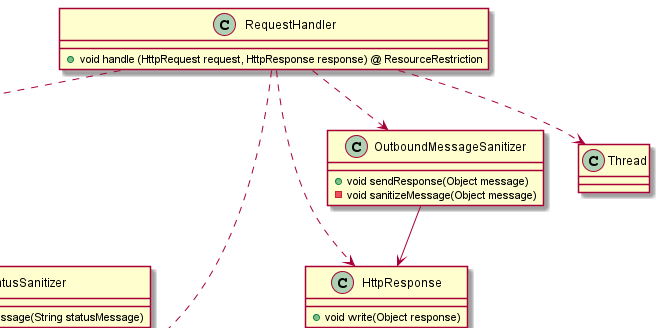
\includegraphics[width=\linewidth]{figure/toyexamples/resource_restriction.png}
    \caption
        [Applying constraint 5 to BlogWeb]
        {Applying constraint 5 to the model of BlogWeb using the added annotation on the RequestHandler class.}
    \label{fig:toy_resource_restriction}
\end{figure}




\section{Extending ArchUnit analysis}

In the current ArchUnit API, a rule that aims to constrain method calls can only be defined in terms of the signatures of the method and its parameters. This is not an issue when the arguments passed to a method are of the same type as the parameters. However, the argument might also be a descendant of the parameter type. There is currently no support in ArchUnit to constrain the types of the objects that are actually being passed as arguments.

Consider constraint 7, which aims to ensure that no secrets are passed to the logger. Say there is a \texttt{Secret} annotation that marks all the classes whose instances must not be passed to the logger. An attempt can be made to enforce the constraint with the current ArchUnit API using a custom predicate, as seen in Listing~\ref{lst:constraint_6_attempt}. Given that a typical logger will accept either a plain string, or a format string along with an array of objects to be formatted, this architectural rule does little in the way of preventing secrets from being passed to such a logger.

\begin{minipage}{\linewidth}
\begin{lstlisting}[caption={A first attempt to implement constraint 7.}, captionpos=b, label=lst:constraint_6_attempt, numbers=left]
ArchRule doNotLogSecrets(Class<?> logger) {
    return noClasses()
        .should().callMethodWhere(
            parameterTypeAnnotatedWith(Secret.class)
                .and(targetOwner(type(logger)))
        );
}
\end{lstlisting}
\end{minipage}

For the final 2 constraints, there is a need for an extension that allows constraints to be defined against method arguments rather than parameters. There should also be hints about where these arguments have been derived from, e.g. which types that make up the components of a concatenated string. The following sections describe the extensions that have been made to ArchUnit, both in regards to its analysis and the information represented in its domain, as well as how these extensions are utilized in the definitions of the final constraints.

\subsection{Implemented extensions}

\textbf{Background.} ArchUnit builds its representation of the architecture using ASM\footnote{\url{https://asm.ow2.io/}}, a Java bytecode analysis framework. ASM reads bytecode and generates callbacks to methods in its various visitor classes. 
The visitor of most interest to us is \texttt{MethodVisitor}\footnote{\url{https://asm.ow2.io/javadoc/org/objectweb/asm/MethodVisitor.html}}, which is responsible for processing the contents of a method, constructor or static initializer. These are collectively named \textit{code units} in ArchUnit's domain, i.e. anything that may contain code.

ArchUnit extends the \texttt{MethodVisitor} class in \texttt{MethodProcessor}, which primarily visits instructions related to field accesses and method invocations (see Figure~\ref{fig:method_processor_1}). These instructions are processed into information about accesses between Java members, not entirely unlike the information provided by a static call graph.

\begin{figure}[H]
    \centering
    \captionsetup{justification=centering}
    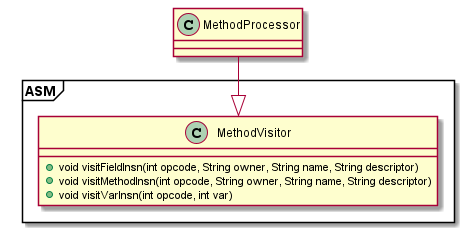
\includegraphics[width=0.6\textwidth]{figure/extension/MethodProcessor1.png}
    \caption
        [ArchUnit: The context of the \texttt{MethodProcessor} class]
        {ArchUnit: The immediate context of the \texttt{MethodProcessor} class, responsible for analyzing code units.}
    \label{fig:method_processor_1}
\end{figure}

Java, as a stack-oriented programming language, passes arguments to method calls and field assignments via the operand stack \cite{hutchison_information_2005}. As such, an inspection of the operand stack at the time of a method call yields information about the arguments being passed.
Conveniently, ASM provides an extension of its \texttt{MethodVisitor} class, called \texttt{AnalyzerAdapter}, which is capable of simulating the effect that each instruction has on the operand stack.

\textbf{SecArchUnit.} As seen in Figure~\ref{fig:method_processor_2}, \texttt{MethodProcessor} now extends \texttt{Analyzer\-Adapter} and utilizes the information about the operand stack to perform an analysis of information flow within a code unit.

\begin{figure}[ht]
    \centering
    \captionsetup{justification=centering}
    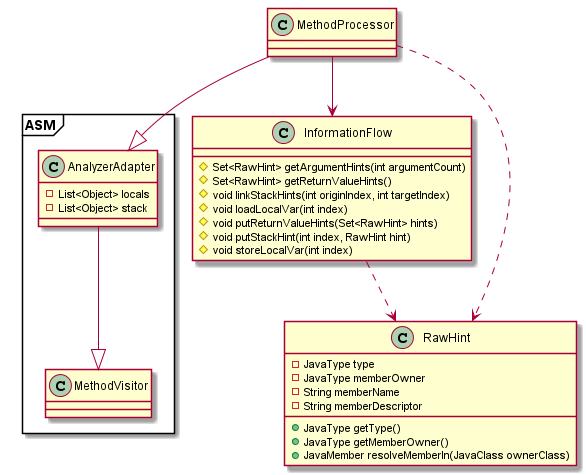
\includegraphics[width=0.7\textwidth]{figure/extension/MethodProcessor2.png}
    \caption
        [SecArchUnit: Changes made to the analysis of code units]
        {SecArchUnit: Changes made to the analysis of code units.}
    \label{fig:method_processor_2}
\end{figure}

The information flow analysis of a code unit, which lends ideas from \cite{hutchison_information_2005}, can be boiled down to the following key points:

\begin{itemize}
    \item Loading a field onto the stack yields a hint in that stack position about its originating member, i.e. the field.
    \item Invoking a method that has a return value yields a hint in the stack position of the resulting object about its originating member, i.e. the invoked method.
    \item Invoking a static method transfers the hints about the arguments, if any, into the stack position of the resulting object, if the method has a return value.
    \item Invoking a non-static method additionally transfers the hints about the arguments into the instance the method was invoked on, and the hints about the instance into the resulting object.
    \item Storing an object in an array transfers the hints about the object into the array.
    \item Loading an object from an array transfers the hints about the array into the object.
    \item Storing or loading a local variable transfers the hints from the stack to the local variable and vice versa.
    \item Duplicating a reference also duplicates the collection holding the hints for that reference, such that hints that flow into the duplicate also flow into the original reference.
\end{itemize}

Once the analysis of all classes has been completed and SecArchUnit has built its representation of the architecture, the raw hints are resolved into hints referencing the actual type (\texttt{JavaClass}) and its origin (\texttt{JavaMember}), if any. As seen in Figure~\ref{fig:domain_changes_1}, \texttt{JavaAccess} now contains hints about the references that flow into the arguments of a method call or field assignment. Additionally, \texttt{JavaMethod} contains hints about the references that flow into the return value of the method. These changes to the domain aim to facilitate the definition of rules that constrain information flow.

\begin{figure}
    \centering
    \captionsetup{justification=centering}
    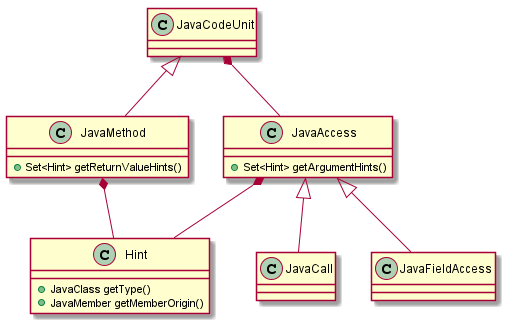
\includegraphics[width=0.7\textwidth]{figure/extension/DomainChanges1.png}
    \caption
        [SecArchUnit: Changes made to the domain surrounding code units]
        {SecArchUnit: Changes made to the domain surrounding code units.}
    \label{fig:domain_changes_1}
\end{figure}

\subsection{Constraint 6: Sensitive information must stay within trust boundary}
% Description
The rule definition for constraint 6 is presented in Listing~\ref{lst:constraint_6_impl}.
This constraint aims to restrict how assets that consist of sensitive information are allowed to flow between classes. The constraint deals with the two concepts of assets and asset handlers, which are expressed in the form of \texttt{Asset} and \texttt{AssetHandler} annotations in the source code. An asset is a sensitive member that should only flow to classes marked with a high security level, i.e. an asset handler.

\begin{minipage}{\linewidth}
\begin{lstlisting}[caption={Rule definition for constraint 6.}, captionpos=b, label=lst:constraint_6_impl, numbers=left]
ArchRule doNotBleedAssetsBetweenComponents() {
    return fields()
        .that().areAnnotatedWith(Asset.class)
        .should(notBleedToInsecureComponents);
\end{lstlisting}
\end{minipage}

% Rule definition
The rule itself requires no arguments, as all the necessary information is injected into the source code in the form of annotations. The custom condition, \texttt{notBleedTo\-InsecureComponents}, ensures that the asset is only accessed directly by asset handlers. Moreover, it utilizes the information about information flow to ensure that the asset is not accessed indirectly through calls to methods where the asset flows into the return value. Its full definition can be seen in Listing~\ref{lst:constraint_6_condition}.

The concept of asset handlers is treated as a single group of classes that have to a high security level, and are therefore granted access to all assets. No distinction is made between different assets and asset handlers in the current implementation.

% Applied to toy app
In BlogWeb, the \texttt{password} field is considered an asset that must stay within the trust boundary of \texttt{UserLoginRequest} and \texttt{UserAuthenticator}. The appropriate annotations in this scenario can be seen in Figure~\ref{fig:assets_toy_system}.

\begin{figure}[ht]
    \centering
    \captionsetup{justification=centering}
    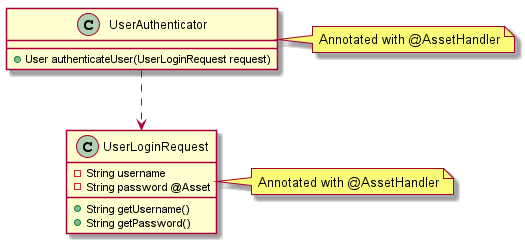
\includegraphics[width=0.8\textwidth]{figure/toyexamples/Assets.png}
    \caption
        [Application of constraint 6 to BlogWeb]
        {Application of constraint 6 to BlogWeb.}
    \label{fig:assets_toy_system}
\end{figure}

\subsection{Constraint 7: Secrets must not be exposed in log messages}
% Description
The rule related to constraint 7, which dictates that secrets must not be exposed in logs, is defined in Listing~\ref{lst:constraint_7_impl}.
There are a multitude of ways that a secret field can be exposed in a log message, e.g. through string concatenation, string formatting, or wrapping it in a different object and converting that object to its string representation. What these exposures have in common is that they issue a method call to the logger where the secret has flowed into the method arguments.

\begin{minipage}{\linewidth}
\begin{lstlisting}[caption={Rule definition for constraint 7.}, captionpos=b, label=lst:constraint_7_impl, numbers=left]
ArchRule doNotLogSecrets(
        DescribedPredicate<? super JavaClass> loggerDescriptor) {
    return noClasses()
        .should(passSecretArgumentTo(
            targetOwner(loggerDescriptor)
        ));
\end{lstlisting}
\end{minipage}

% Rule definition
Rather than a single class representing the preferred logger, as in constraint 1, this constraint should prevent exposures through all loggers present in the system. Therefore, the rule accepts a predicate that should select all such logging facilities. The custom condition \texttt{passSecretArgumentTo} inspects the argument hints of all outgoing method calls for any members marked with the \texttt{Secret} annotation. Additionally, for each originating member found in the hints, it recursively checks the hints that have flowed into that member, in an attempt to constrain information flow with intermediate steps in different code units.

% Applied to toy app
In BlogWeb, the constraint can be applied as seen in Listing~\ref{lst:constraint_7_rule}. The only secret in this system is the password field, annotated in Figure~\ref{fig:secrets_toy_system}.

\begin{minipage}{\linewidth}
\begin{lstlisting}[caption={Application of constraint 7 to BlogWeb.}, captionpos=b, label=lst:constraint_7_rule, numbers=left]
@ArchTest
ArchRule doNotLogSecrets = SecArchUnit
    .doNotLogSecrets(type(Logger.class));
\end{lstlisting}
\end{minipage}

\begin{figure}[H]
    \centering
    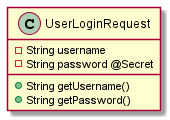
\includegraphics[width=0.25\textwidth]{figure/toyexamples/Secrets.png}
    \caption
        [Annotation added to BlogWeb for constraint 7]
        {Annotation added to BlogWeb for constraint 7.}
    \label{fig:secrets_toy_system}
\end{figure}